\chapter{Implementación}

En este capítulo se procede a desarrollar cada uno de los PMV de cara a cada hito relacionado con 
la implementación, los primeros hitos se han dedicado a definir la infraestructura y organización del 
proyecto. De manera que los siguientes hitos se irán definiendo uno tras otro, debido a que el enfoque 
interactivo, principio fundamental del desarrollo ágil, no permite una planificación amplia. Por lo que no 
se podrían establecer todos los PMV desde el principio, además, habrá que discutir qué herramientas van a usarse 
para desarrollar o llevar a cabo estos hitos y el porqué de su elección. 

Primeramente, se decidirá en este caso qué herramienta se usará para albergar el proyecto y poder definir los 
hitos, además de permitir un seguimiento del desarrollo mucho más controlado, siguiendo así con el enfoque ágil 
visto en el primer capítulo. Tras ello se irá desarrollando cada PMV siguiendo las mejores prácticas posibles y 
obteniendo un producto de calidad, principios afines de nuevo al enfoque ágil.


\section{M0: Configuración inicial del TFG - Creación del repositorio}

Ya que el desarrollo avanza a base de productos mínimamente viables, lo primero que se
debe hacer es definir un repositorio en el que definir estos hitos. Por ello es la primera herramienta
que se va a elegir. Teniendo en cuenta el uso de git como sistema de control de versiones debido a que es 
la herramienta de control de fuentes más usada genéricamente. 

Teniendo esto presente, se busca un repositorio basado en git que albergue el proyecto. Además, se busca
una herramienta online y gratuita, por lo que se encuentran varias opciones basadas en git que cumplen estas
medidas, como por ejemplo GitHub \footnote{\url{https://github.com/}}, GitLab
\footnote{\url{https://about.gitlab.com/}} y Bitbucket \footnote{\url{https://bitbucket.org/}}, 
plataformas de desarrollo colaborativo que comparten muchas características. 

En general, las versiones gratuitas de estas plataformas son adecuadas para muchos proyectos pequeños y
medianos, al menos las de GitHub y GitLab. Por ello, la elección entre una de estas plataformas depende de 
otros factores, ya que son herramientas muy parecidas, y cualquiera de estas herramientas cumple los criterios
para su elección.

Es por esto que la herramienta elegida será GitHub debido a la familiaridad que se tiene con esta herramienta y 
por ende la comodidad de su uso \footnote{\url{https://github.com/JoseJordanF/Claqueta}}.

Para proseguir con el enfoque sobre la calidad del proyecto, y su control sobre cada cambio en el proyecto, apuntando 
en este caso a la documentación, se necesita un flujo de trabajo para verificar la ortografía y la gramática de la 
documentación del proyecto. Por ello se hace uso de GitHub Actions una herramienta de integración continua integrada 
en GitHub. Esta herramienta ofrece una guía para crear los flujos de trabajo necesarios, en este caso un verificador 
ortográfico y gramatical, también se aprovechará para crear otro flujo que compile la documentación LaTeX. Debido a 
que es una herramienta con la que se está familiarizado, al igual que con GitHub, es mucho más cómodo su uso, de 
manera que será bastante sencilla la creación de estos flujos de trabajo. 

Una vez se ha escogido el repositorio y se han creado los flujos hasta ahora necesarios, se puede dividir 
la implementación del software en hitos. Estos han sido definidos en GitHub y cada uno de ellos contiene un grupo de 
\textit{issues} que sé corresponden con las distintas mejoras que se han ido incorporando al proyecto a lo largo
de su desarrollo.

El uso de herramientas permite llevar a cabo el proyecto, asegurando tanto su calidad, como el seguimiento de buenas
prácticas durante el uso de estas, velando por el enfoque iterativo del proyecto, su adaptabilidad y flexibilidad;
principios ágiles, imprescindibles durante el desarrollo del proyecto, ajustándose estas herramientas a cada
uno de los hitos y adaptándose también a los posibles cambios durante el desarrollo. Para ello se describirán las
herramientas usadas para el desarrollo de cada hito, justificando su elección bajo ciertos criterios, explicándose 
por qué han sido elegidas.

\section{M1: Definición de objetos - Abstracción del dominio del problema}

En este hito \footnote{\url{https://github.com/JoseJordanF/Claqueta/milestone/8}} se conseguirá el 
modelado de los objetos presentes en el problema, para ello se abstraerán 
los conceptos clave y se definirán los objetos de la aplicación. El objetivo es tener una estructura 
clara de los datos a utilizar. La abstracción permite identificar las características 
esenciales, eliminando detalles innecesarios. La definición de objetos ayudará a comprender sus 
relaciones, atributos y operaciones. Esto establecerá una base sólida para el desarrollo coherente 
de la aplicación.

De esta manera se busca priorizar el desarrollo real, la retroalimentación continua y prácticas como 
el desarrollo impulsado por pruebas \begin{otherlanguage}{english}\textit{(Test Driven Development, TDD)}\end{otherlanguage}  ,y la colaboración cercana. Esto permite una mayor 
agilidad y adaptabilidad en el proceso de desarrollo.

Por ello, se busca un método para definir los objetos de la aplicación, se encuentra una técnica de 
desarrollo de software llamada, \begin{otherlanguage}
{english}``\textit{\textbf{Domain Driven Design}}''\end{otherlanguage}(DDD) \cite{NvDDD} es un enfoque 
de diseño de software que se centra en comprender y modelar el dominio del problema de una aplicación. 
Busca desarrollar un diseño que refleje con precisión las reglas y conceptos del dominio, lo que 
resulta en un sistema más mantenible. Teniendo en cuenta que el DDD y el desarrollo ágil son 
compatibles, ya que su aplicación permite construir aplicaciones que se ajusten mejor a las necesidades 
del cliente y evolucionen de manera flexible a medida que se adquiere un mayor entendimiento del 
dominio. DDD proporciona la base conceptual y un diseño sólido para desarrollar modelos de dominio 
claros y significativos, mientras que el enfoque ágil permite una implementación iterativa, rápida y 
adaptativa.

De esta manera se recurre al uso del \textit{\textbf{modelo de dominio}} representación conceptual de 
las entidades, los conceptos, las reglas, los objetos inmutables, como los objetos valor y las 
interacciones dentro del dominio del problema. Es una abstracción del mundo real que captura las 
principales entidades y sus relaciones. Esto ofrece una gran ventaja del DDD, ya que esto ayuda a 
alinear el entendimiento y facilita la comunicación efectiva sobre el problema y su solución. Siendo 
los modelos de dominio una parte central y fundamental del DDD, representando el conocimiento y la 
comprensión profunda del problema que se está abordando. Teniendo esto en cuenta se crea un modelo de 
dominio.

\begin{figure}[h]
    \centering
    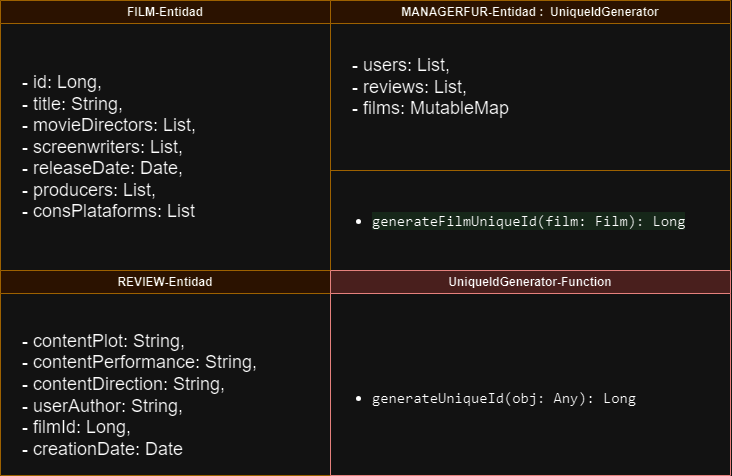
\includegraphics[width=\linewidth]{imagenes/Modelo_Dominio_Claqueta_TFG.drawio.png}
    \caption{Modelo de dominio.}
    \label{fig:diagrama}
\end{figure}



Como base y resumen del modelo de dominio, se tiene una entidad \begin{otherlanguage}
{english}\textit{\textbf{review }}\end{otherlanguage}haciendo referencia a la reseña, la entidad 
esencial, ya que se persigue asegurar la calidad de esta. Una reseña de calidad va a ser definida 
comúnmente como una reseña fiable que cumpla las reglas que se vieron en el estado del arte. Por lo tanto, 
estará formada por atributos generales como un identificador que la relacione con la 
película a la cual está criticando y otro para identificar al usuario que la ha escrito, la fecha de 
realización de esta crítica y también el contenido de la reseña se dividiría para que el usuario hable tanto de la 
trama general, la interpretación y la dirección. Asegurando las reglas vistas en el estado del arte.

Otra entidad importante es la \begin{otherlanguage}{english}\textit{\textbf{film }}\end{otherlanguage} 
siendo su propuesta mínima un conjunto de atributos que definen el contenido de dicha película como los 
directores, los guionistas, la fecha de estreno, las productoras y las plataformas en las que se puede 
consumir dicha película. Este conjunto de atributos es indispensable para la recomendación de dicho 
contenido, siendo cada uno puntos en común que buscar en otras películas para sus recomendaciones 
personalizadas. Evidentemente, también se necesita el título de la película y un identificador, ya que el 
resto de atributos puede coincidir y no identificar de manera única a la película.

Por último, existe una entidad que se encarga de gestionar tanto películas, como reseñas, como 
usuarios. Además, hace uso de una función que nos permitirá generar el identificador único para cada 
película y otros objetos que lo puedan necesitar.

\subsection{Lenguaje de programación}

Una de las principales herramientas para el desarrollo de software es el lenguaje de programación, un 
lenguaje que sea afín a las necesidades del proyecto. Siendo así necesario un lenguaje para modelar 
los objetos descritos en este capítulo, en el primer hito. Pero hay que tener en cuenta que se pretende 
que el desarrollo del modelado de los objetos pueda ser reutilizable, de fácil acceso e intentando 
ahorrar recursos. Por ello, se podría diseñar una API propia, como las que se 
mencionaron en el capítulo del estado del arte. Ya que es muy atractivo que los algoritmos y el modelo 
de datos pueda ser consumido por otros a través de una API

Por ahora se debe encontrar un lenguaje que sea flexible y que se adapte a las necesidades del proyecto. Con 
lo que se busca un lenguaje de propósito general, lo cual permitirá crear diversos proyectos. 
Siendo estos más sencillos de implementar en unos lenguajes que en otros. Se podría pensar en lenguajes 
como Java, Groovy, Scala o Kotlin. Siendo todos ejecutados en la máquina virtual de java (JVM), siendo 
Java, el veterano, es robusto y multiplataforma, pero su sintaxis puede ser un tanto prolija. Kotlin, 
por su parte, destaca por ser moderno, conciso y compatible con Java, además de ofrecer avanzadas 
características de seguridad. Aunque Groovy simplifica la sintaxis, su velocidad de ejecución más lenta 
podría ser un inconveniente. Scala, con un enfoque en la programación funcional, es expresivo, pero 
puede presentar una curva de aprendizaje más pronunciada. En conclusión, Kotlin emerge como la elección 
óptima en la JVM debido a su curva de aprendizaje suave, su amplia gama de bibliotecas y su excepcional 
interoperabilidad con Java, presentando una combinación equilibrada de simplicidad y funcionalidades 
avanzadas. 

\subsection{Testing}

Un proyecto con un enfoque ágil está sujeto a pruebas constantemente, algo que se está apegando en este 
proyecto a los PMVs resultantes de los milestones. De esta manera, se asegura la 
calidad del producto y se cerciora su funcionamiento. Consiguiendo así productos de 
calidad más robustos y minimizando errores.

Como se ha mencionado, Kotlin goza de acceso a un extenso conjunto de librerías y \textit{frameworks}. 
En este conjunto existen varios \textit{frameworks} que nos permiten testear el código.

Una herramienta esencial para fortalecer el proceso de desarrollo, las pruebas de flujo de trabajo con Docker 
\cite{GI_act}. Esta herramienta permite llevar a cabo pruebas exhaustivas de los flujos de trabajo de manera 
local antes de su implementación en el entorno remoto, destacándose por su integración efectiva con Docker. La 
característica distintiva de esta herramienta radica en dicha capacidad para generar simulaciones precisas, 
lanzando y evaluando flujos de trabajo en un entorno controlado basado en Docker. Asegurando la funcionalidad y 
consistencia de los flujos de trabajo antes de su inclusión en el entorno remoto, proporcionando la confianza 
necesaria en la calidad del código. Siendo una herramienta clave para garantizar una implementación sin 
contratiempos, mejorando la robustez y la calidad de los flujos de trabajo antes de su despliegue.

Para test unitarios del código existen varios \textit{frameworks}, por un lado,  
\textit{Spek}\footnote{\url{https://github.com/spekframework/spek}}. Una herramienta escrita para 
Kotlin diseñada para facilitar la escritura y ejecución de pruebas en proyectos escritos en este 
lenguaje. Permite definir pruebas en un estilo legible similar al lenguaje natural, lo que facilita 
su comprensión tanto para desarrolladores como para no desarrolladores. Por ello, algunos 
desarrolladores lo relacionan con \begin{otherlanguage}
{english}\textit{Behavior-Driven Development}\end{otherlanguage} (BDD), desarrollo guiado por 
comportamiento. Aunque sus creadores ya han mencionado 
\footnote{\url{https://spekframework.github.io/spek/docs/latest/}} que creen que hay una falsa 
distinción en torno al desarrollo guiado por comportamiento (BDD) y el desarrollo guiado por pruebas 
(TDD). Por lo que recomiendan que se piense en Spek como un simple \textit{framework} de 
especificación.

También se dispone de la herramienta por defecto que incorpora cualquier tipo de proyecto Kotlin, 
\textit{JUnit5}. Este es la última versión del \textit{framework} de pruebas unitarias para Java. Posee 
una arquitectura modular que se compone de tres módulos principales: JUnit Platform, JUnit Jupiter y 
JUnit Vintage, el primero es el núcleo de la herramienta, el segundo introduce las anotaciones y 
permite configurar los test, y la última permite la compatibilidad con versiones anteriores de este 
\textit{framework}. Este es el más usado actualmente por los desarrolladores 
\footnote{\url{https://www.jetbrains.com/es-es/lp/devecosystem-2022/testing/}} como nos indica 
\textbf{\textit{Jetbrains}}, compañía que ha diseñado Kotlin.

Ambos son buenas herramientas de pruebas. Además, permiten la integración con otras bibliotecas o 
\textit{framework} de pruebas. Pero ambas herramientas necesitan de otras bibliotecas imprescindibles 
en las pruebas, estas permiten simular objetos de una clase para trucar el resultado de ciertas 
funciones que se quieran testear. Estos objetos se denominan \textbf{\textit{Mock}}, en Kotlin 
se encuentra la librería nativa \textit{mockk}. Con uno de los \textit{frameworks} 
mencionados y esta librería se podrian realizar los test unitarios que se necesiten. Por lo que principalmente 
si no en su totalidad se usara Junit5 debido a la cantidad de información y ejemplos de uso, además de 
ser la herramienta usada por la mayoría de desarrolladores.

Para la parte de testeo de UI existe acceso a varias herramientas, pero se usará el 
\textit{framework} \textbf{\textit{Espresso}}\footnote{\url{https://developer.android.com/training/testing/espresso?hl=es-419}}, una herramienta creada por Google y la más recomendada \cite{UITest}.

Por último, si fuera necesaria una herramienta para testear las operaciones de una API, para  recuperar, 
insertar, modificar o eliminar información. Como se ha visto entre 
las herramientas más usadas para las pruebas\footnote{\url{https://www.jetbrains.com/es-es/lp/devecosystem-2022/testing/}} se encuentra \textit{\textbf{Postman}} una página para ayudar a los 
desarrolladores de API. Por ello es la herramienta que se usara en tal caso para realizar dichas 
pruebas, además es sencilla y cómoda de usar.

\section{M2: Lógica de negocio - Operaciones sobre los datos}

En este hito \footnote{\url{https://github.com/JoseJordanF/Claqueta/milestone/3}} se hablará de la 
lógica de negocio, también conocida como reglas de negocio, estas se refieren a las operaciones y procesos 
fundamentales que definen cómo funciona la aplicación. Determinando como se procesan los datos, se 
realizan cálculos, se toman decisiones y se llevan a cabo las operaciones clave para lograr los 
objetivos de la aplicación. Siempre dependientes de las necesidades y los propósitos de la aplicación. 
Estas vienen definidas por las \textbf{Historias de Usuario}, por lo que se va a recurrir a ellas para 
determinar las operaciones que se llevaran a cabo sobre los datos. Se promoverá la correcta 
implementación de la lógica de negocio, asegurando la coherencia y validez en las operaciones a través 
de los test unitarios. Siguiendo como siempre la esencia del desarrollo ágil, asegurando las
buenas prácticas para garantizar la calidad del proyecto, teniendo en cuenta que la lógica de negocio es 
el núcleo esencial que da vida a una aplicación y hace posible su funcionalidad y utilidad. 

Cabe destacar que lo primero que se hará es crear un proyecto Kotlin creado por gradle, un sistema de 
automatización de construcción de código de software por defecto, en este caso en IntelliJ IDEA. Esto 
es imprescindible, ya que para una mayor comodidad en la configuración y el uso de las distintas 
herramientas que nos ofrece Kotlin es necesario la creación de un proyecto.

Por otro lado, se necesita un flujo de trabajo que permita seguir unas buenas prácticas comprobando
la calidad del código escrito en dicho lenguaje. Cada cambio, cada nueva incorporación al código, asegurando
su calidad, velando por los principios del enfoque ágil, mencionados en el primer capítulo. Para ello se busca un 
linter o analizador estático de código, siendo este una herramienta que revisa el código en busca de posibles 
errores, malas prácticas o incumplimientos de estilo antes de que se ejecute. Este enfoque proactivo no solo 
ayuda a prevenir problemas antes de que afecten el rendimiento o la funcionalidad del software, sino que 
también se alinea perfectamente con los principios ágiles al fomentar la iteración continua y la mejora 
constante del código, promoviendo así un desarrollo más ágil y eficiente. 

Para la creación de este flujo de trabajo se necesita un linter para Kotlin que compruebe los ficheros con 
extensión de archivo Kotlin(.kt). Y hacer esto cada vez que se añada un nuevo archivo Kotlin al repositorio 
o se modifique alguno ya existente en algún pull request. Para esta tarea es mucho más rentable usar GitHub 
Actions, ya que debido a su amplia comunidad es sencillo encontrar un linter para el lenguaje que se prefiera. 
Por otra parte, la creación del flujo es prácticamente instantánea debido a la guía por parte de GitHub y el conocimiento previo que se tenía de estos al haber usado antes dicha herramienta. 
También es una tarea sencilla y poco pesada para que GitHub Actions la lleve a cabo, y no ocasiona gastos 
adicionales.
A continuación, cada una de las siguientes secciones representa un conjunto de issues que se han resuelto para obtener 
un PMV.

\subsection{Identificación y creación de las películas}

Una vez creado el proyecto con los modelos de dominio, se comienza a pensar en las 
distintas operaciones sobre los datos. Para empezar se debería preguntar qué contenido van a 
consumir los usuarios, claramente películas y en sí las reseñas de estas. Por lo tanto, primeramente 
hay que diferenciar de manera única cada película. Para ello es necesario el identificador de cada 
película, pero aún no se ha definido como se creara dicho identificador. Para generar este 
identificador se puede optar por múltiples opciones, se podría pensar en usar el título de la película 
o el nombre de alguno de los directores. Pero esto lleva a un problema debido a 
que existen películas que poseen el mismo título y son diferentes, al igual que los directores. 
Incluso se puede llegar a dar la casualidad de que existan dos películas con el mismo título y 
un director en común, siendo estas diferentes. Por lo tanto, no se podría usar el título y algún 
director, o al menos si solo se usan estos datos. Por lo tanto, esta deja de ser una posibilidad, aún 
hay muchas más opciones, se podría recurrir a la base de datos para generar un identificador 
único, ya que muchas bases de datos modernas poseen esta función incorporada. Pero no se quiere 
depender de la base de datos para generar estos identificadores, ya que en este punto del proyecto no 
es necesaria la base de datos. De manera que existen otras opciones como GUID una implementación de 
Windows para generar identificadores siguiendo un algoritmo específico, o alguna otra opción como los 
métodos que usan una marca en el tiempo y un identificador para cada nodo en el sistema. La comparación 
entre ambas opciones \cite{compSnowUUID} deja ver que las opciones estilo UUID son valores de 128 bits 
y no tienen un criterio determinado para generar dicho identificador, mientras que los métodos estilo 
snowflake son valores enteros de 64 bits y tienen una forma determinada de generar dicho identificador. 
Debido a la facilidad de seguir un algoritmo determinado y que no se necesita representar demasiados 
datos como para usar 128 bits, se ha decidido usar snowflake \cite{snowF} método creado por Twitter. 
Básicamente, se basa en crear un identificador único representado en decimal por número binario creado 
por bloques, el primero de 41 bits que define los milisegundos pasados desde una marca de tiempo 
determinada, el segundo bloque de 10 bits representa un identificador propio del objeto, en este caso 
se ha decidido fusionar el título de la película y el nombre del primer director para crear un número 
de 10 bits para este bloque. Por último, el bloque final de 12 bits que simplemente represente un 
número de secuencia por si se da la casualidad que se crean varios objetos en el mismo milisegundo y 
con el mismo título y primer director. Dándonos un identificador que cumple con las necesidades de 
sobra.

\subsection{Que es el consumo, quién lo consume y como lo lleva a cabo}

Tras resolver este problema para identificar el contenido, se puede pasar a definir como crear ese 
contenido por parte de la entidad que administra todo. Para ello, cada vez que se crea una película, 
además de introducir todos los datos requeridos, se crea su identificador y se añade a la lista de 
películas del proyecto. Ahora bien, para que este contenido pueda ser consumido por los usuarios, estos
deben estar creados en el sistema, por tanto, se define como se crea un usuario y se introduce 
en la lista de usuarios. Esto lleva a responder como se define el consumo y como se designa que un 
usuario ha consumido, en este caso una película. Lo que lleva a una interacción por parte del 
usuario para responder a esas preguntas, definiéndose ese consumo como la creación de reseñas por parte de este.
Siendo las películas en las que reseña o en las que interactúa con las reseñas de alguna manera, las películas que 
consume el usuario. Esto es algo que se definirá más adelante en la lógica de negocio. 

\subsection{Creación de reseñas}

Una vez creadas las películas y los usuarios, se necesita definir como se crean las reseñas a través de 
los datos necesarios, la relación con la película y el usuario que la ha escrito. Ya que se tiene todo 
lo necesario para la creación de esta reseña. Dando lugar a la reseña en sí misma y a la marca del 
consumo por parte del usuario, tema mencionado justo en la sección anterior. Además de comprobar que no 
exista una reseña de esa película ya escrita por este usuario, ya que cada usuario solo puede escribir 
una reseña por película.

\subsection{Recomendación de contenido al usuario}

Definido el consumo como la realización de reseñas por parte del usuario, se toma esto como marca 
de consumo. Siendo el consumo del usuario, todas las películas en las que ha 
reseñado estas servirán para la creación de sus recomendaciones. Las recomendaciones 
se harán a través de los datos comunes de estas películas, los directores, las productoras, los guionistas o las 
plataformas donde se pueden ver estas películas. Cualquiera de estos datos se utilizará para recomendar cualquier 
película que no se haya consumido y tenga algún dato en común con el consumo del usuario. De esta manera 
se obtendría una lista de películas recomendadas para el usuario sin repetidos, ya que es posible que varios datos 
coincidan en las mismas películas. Esta lista se refrescará cada vez que el usuario escriba una reseña 
en una nueva película.

Por cada una de estas operaciones se pueden dar varios casos de uso que se han estudiado a través de 
los test unitarios. Comprobando que cada caso de uso se lleva a cabo como se espera y el conjunto de 
ellos también. Para proseguir con las buenas prácticas y asegurar la calidad del proyecto y de su desarrollo, 
se deben seguir los principios vistos en la introducción sobre enfoque ágil, proporcionando una calidad mayor al 
proyecto y obteniendo un mayor control sobre su desarrollo. Es por esto que se debe crear un flujo de trabajo 
que permita la ejecución de los test unitarios cada vez que se realice un cambio en los ficheros Kotlin del 
proyecto. Por lo tanto, es necesario decidir que herramienta de integración continua se va a usar para ello. 
GitHub Actions puede usarse perfectamente para la creación del flujo, al igual que se usó para el flujo del 
linter, ya que solo se necesita ejecutar test unitarios simples que pueden ser ejecutados en una máquina virtual 
Ubuntu y en este caso para asegurar el correcto funcionamiento de estos, son ejecutados sobre distintas 
versiones de Java.

\section{M3: Servicios esenciales para la aplicación}

En este hito \footnote{\url{https://github.com/JoseJordanF/Claqueta/milestone/9}} se busca dotar a la aplicación de
dos funcionalidades esenciales para esta, siguiéndose el problema planteado por el desarrollador 
\footnote{\url{https://github.com/JoseJordanF/Claqueta/issues/125}}. De esta manera, primero se debe buscar una 
herramienta para el primer servicio, que según lo expuesto por el desarrollador, debe ser una herramienta que 
permita gestionar la configuración de la aplicación; pudiéndose obtener lo necesario para el arranque de la aplicación 
y su posterior funcionamiento. Esta herramienta debe ser capaz de cargar esta configuración desde distintas fuentes, 
velando por el arranque de la aplicación, ya que como menciona el desarrollador, estos ficheros pueden ser de 
distintos tipos, luego afiliarse a uno solo podría llevar a una carga errónea de este y que la 
aplicación no funcionase. Por lo que se ha recurrido a las fuentes más populares en aplicaciones Kotlin 
\cite{popularConfig} como JSON\cite{JsonWiki}, ficheros Java Properties\cite{JProWiki}, YAML\cite{YmlWiki}, 
HOCON\cite{HoconWiki} o ficheros INI\cite{IniWiki}. Esta sería una de las fuentes independientemente del tipo de 
archivo, otra indudable fuente y más habitual, son las variables de entorno, aunque en lenguajes de la JVM como 
Kotlin aparece otra fuente similar a las variables de entorno; en este caso se trata de las propiedades
del sistema, en sí de la JVM 
\footnote{\url{https://docs.oracle.com/javase/tutorial/essential/environment/sysprop.html}}. Con estas tres fuentes
se puede crear una jerarquía de lectura según las practicas más habituales en los lenguajes de la JVM 
\footnote{\url{https://docs.appdynamics.com/appd/4.5.x/en/application-monitoring/install-app-server-agents/java-agent/administer-the-java-agent}}, en este caso en Kotlin, así se seguirá la siguiente jerarquía, la primera fuente 
será las variables de entorno del sistema, si esta falla se recurrirá a las propiedades del sistema 
\cite{SecrectsJavaP} y por último se recurrirá al archivo de configuración.

Para Kotlin existen mucha variedad de bibliotecas para controlar la configuración de la aplicación, pero se busca 
una que permita el máximo número de fuentes vistas antes, e incluso que permita leer variables de entorno y archivos 
dotenv. Se busca principalmente en el repositorio oficial de Maven \footnote{\url{https://mvnrepository.com/}}, ya 
que brinda una gran cantidad de opciones, además de más información relacionada con la popularidad de la biblioteca 
o las vulnerabilidades que estas tienen. Las bibliotecas encontradas serían las siguientes, Apache Commons 
Configuration\footnote{\url{https://commons.apache.org/proper/commons-configuration/}}, Config de 
Lightbend\footnote{\url{https://github.com/lightbend/config}}, Config 
Magic\footnote{\url{https://github.com/brianm/config-magic}}, Config de 
NetworkNT\footnote{\url{https://mvnrepository.com/artifact/com.networknt/config/2.1.33}}, están listadas en orden de
popularidad, la mayoría tiene soporte para leer de distintas extensiones como JSON o YAML, pero pocas pueden leer de
más de una de estas extensiones; sin embargo, Config de Lightbend y  Config de NetworkNT poseen soporte nativo para 
JSON, ficheros Java Properties y JSON, YAML respectivamente. Pero desgraciadamente ninguna de ellas puede leer 
nativamente archivos dotenv, ni variables de entorno, ni propiedades del sistema. Por lo que se ha decidido usar una 
librería creada por el desarrollador\footnote{\url{https://github.com/JoseJordanF/LibraryConfigProject}}, la 
cual encapsula el funcionamiento de tres bibliotecas, una ya se conoce, ya que es una de las mejores opciones 
discutida arriba, Config de Lightbend que cubre JSON, Java Properties y HOCON, dotenv-
java\footnote{\url{https://github.com/cdimascio/dotenv-java}} que cubre las variables de entorno y los archivos 
dotenv y por último snakeyaml \footnote{\url{https://bitbucket.org/snakeyaml/snakeyaml/src/master/}} que cubre los 
archivos YAML. También de forma nativa lee propiedades del sistema y variables de entorno del sistema, de manera que 
dicha librería lee nativamente archivos JSON, Java Properties, YAML, HOCON e incluso dotenv, además encapsula la 
lectura de fuentes indispensables y más habituales, variables de entorno y propiedades del sistema, por ende es la 
herramienta perfecta para la aplicación.

De modo que la implementación de esta funcionalidad constara de una clase \begin{otherlanguage} {english}``\textit{\textbf{configurator}}''\end{otherlanguage} que permita cargar la configuración siguiendo la 
jerarquía comentada, y en cualquier momento permitir obtener dichos datos a través de dicha clase. Se necesita que
solo exista una instancia de esta clase, ya que simplemente se cargara la configuración al inicio de la aplicación, 
sin necesidad de más instancias, aportando control estricto sobre la única instancia, ya que la configuración,
trata con secretos delicados. A este patrón de diseño se le conoce como patrón singleton \cite{PattSingl}, en Kotlin 
existen algunas formas de conseguir esto \cite{SinglKotlin}, en este caso esto se logra marcando el constructor como 
privado, lo que evita la creación de instancias fuera de la propia clase. Además, se utiliza un objeto companion 
para almacenar esta única instancia y proporcionar un punto de acceso global a través de la clase. De esta manera, 
se asegura que cualquier parte del código pueda acceder a la misma instancia de \begin{otherlanguage} {english}``\textit{\textbf{configurator}}''\end{otherlanguage}, garantizando la coherencia de la configuración en 
toda la aplicación.

Para la segunda funcionalidad esencial, tal como menciona el desarrollador 
\footnote{\url{https://github.com/JoseJordanF/Claqueta/issues/126}}, se necesita una herramienta que permita 
registrar las distintas acciones de la aplicación para controlar el correcto funcionamiento de esta, y sobre todo 
los errores que se puedan dar durante su ejecución. También debe permitir el registro de la actividad de las 
acciones del usuario; dando estos registros por pantalla o en un archivo de registros, o incluso en ambos, con un 
formato descriptivo para una lectura clara del registro. En este caso, Kotlin o los lenguajes de la JVM poseen 
varias opciones populares, destacando del repositorio de Maven el módulo 
SLF4J\footnote{\url{https://www.slf4j.org/}}. Este módulo sirve de fachada o abstracción para distintos marcos de 
registro muy populares en estos lenguajes, como LogBack\footnote{\url{https://logback.qos.ch/documentation.html}}, 
Log4j 2\footnote{\url{https://logging.apache.org/log4j/2.12.x/}} o Apache Commons 
Logging\footnote{\url{https://commons.apache.org/proper/commons-logging/}}, siendo estos los más usados y populares 
dentro de la comunidad, tal como nos indica Maven\footnote{\url{https://mvnrepository.com/open-source/logging-frameworks}}. 
De esas tres bibliotecas, LogBack y Log4j 2 cumplen con los requisitos del desarrollador, ya que Apache Commons 
Logging carece de configuración que permita dar un formato específico a los logs o indicar la salida de estos, 
además es una fachada comúnmente usada para redirigir los mensajes de registro a SLF4J. Por lo tanto, cualquier 
biblioteca entre las dos mencionadas con anterioridad cumpliría con los requisitos, aun así la elección se va a 
decantar por LogBack, ya que es un poco más popular y usada que Log4j 2.

La implementación de esta funcionalidad será como la anterior, ya que también será una clase singleton 
\cite{DPatterns} llamada \begin{otherlanguage} {english}``\textit{\textbf{SimpleLogger}}''\end{otherlanguage}, en 
este caso, ya que pueden crearse múltiples implementaciones del logger sin perturbar el código. Siendo una clase 
singleton para tener control sobre la única instancia existente y que sea más eficiente, ya que será más fácil de 
mantener una sola instancia. Esta se encargará de inicializar el objeto responsable de los registros, indicando la 
configuración de la biblioteca, teniendo en cuenta donde se guardaran los logs, como lo harán y en que formato lo 
harán, esto se consigue gracias a una interfaz que permite definir los componentes necesarios en la configuración de 
la biblioteca, los cuales son el \begin{otherlanguage} {english}``\textit{\textbf{appender}}''\end{otherlanguage} y 
el \begin{otherlanguage} {english}``\textit{\textbf{encoder}}''\end{otherlanguage}, el primero es el encargado de 
donde y como guardar los logs, mientras que el segundo indica el formato en el que lo hacen. De esta manera se podrán 
hacer distintas implementaciones de estos métodos para disponer de diferentes tipos de logs.

Por otro lado, también se hace uso de una clase LoggerManager la cual se usa para inyectar la implementación de 
logger que se requiera sin perturbar la implementación en el resto del código. Por último se dará como válida esta
implementación si pasa los test unitarios correspondientes, estos permiten comprobar si sé crean los registros en 
distintas operaciones de la aplicación, de manera que se comprueba su creación y si su información es la que se 
espera. Así se demuestra que las clases que usan el logger lo están usando como deberían y se demuestra que la 
implementación del logger funciona. 

\section{M4: Refactorización para la mejora de prácticas en el manejo de estructuras de datos y errores}

En este hito se pretende realizar una refactorización basada en algunas historias del 
desarrollador,\footnote{\url{https://github.com/JoseJordanF/Claqueta/issues/132}}
estas aseguran un funcionamiento más óptimo de la aplicación mediante el uso de las mejores prácticas sobre las 
estructuras de datos, disminuyendo el número de operaciones, o haciendo que estas sean más eficientes. También por 
parte del desarrollador \footnote{\url{https://github.com/JoseJordanF/Claqueta/issues/129}} se pretende establecer una 
jerarquía de clase para los posibles errores que puedan ocurrir en la aplicación. De esta manera se obtendrá una 
refactorización del código actual en el que se siguen las mejores prácticas en el manejo de estructuras de datos y el 
manejo de errores, siendo este el PMV obtenido tras la validación de este hito

Para mejorar la eficiencia de la aplicación se ha recurrido al uso o al cambio de estructuras de datos, como por 
ejemplo las reseñas, anteriormente estaban localizadas en una lista de objetos \begin{otherlanguage} {english}``\textit{\textbf{Review}}''\end{otherlanguage}, 
pero esto lo hacía tremendamente ineficiente, ya que si se quisieran buscar las reseñas de un usuario o las reseñas 
de una película tendrían que localizarse recorriendo la lista. Pero haciendo uso de un diccionario\cite{OaksJava} que 
relaciona un identificador con un grupo de reseñas es eternamente más eficiente. Para ello se han realizado varios 
cambios, la forma de añadir un usuario comprobando que no existía ya uno con dicho nombre era bastante ineficiente, ya 
que requería recorrer la lista, por lo que se ha decidido usar un conjunto para guardar los usuarios. Así se 
han sobrecargado los métodos de conjunto\cite{BlochEffective} para considerar dos usuarios iguales si tienen el mismo 
nombre de usuario, de manera que agregar nuevos usuarios es más sencillo y más eficiente a la hora de comprobar si ya 
existe alguno con el mismo nombre de usuario.

Una vez hecho el cambio de los usuarios, al crear una reseña ahora se añaden dos entradas a la estructura de datos 
que las contiene, una representa las reseñas realizadas por el usuario y otra las reseñas referentes a una misma 
película. Así se tendría una eficiencia constante al realizar operaciones de búsqueda sobre dicha 
estructura\cite{LaforeData}; también se hace más eficiente la forma de comprobar si un usuario ya ha escrito una 
reseña sobre una película, ya que el conjunto de reseñas afiliado a esa clave del mapa que representa a una película o 
a un usuario, es un conjunto, de modo que también se sobrecargan los métodos del conjunto para designar una reseña 
igual a otra siempre que los identificadores que guarda dicha reseña sean iguales a los de otra. Así se impide la 
adición de reseñas repetidas porque en un conjunto de reseñas referentes a una película o aún usuario no puede haber 
más de una reseña con la misma ID de usuario o la misma ID de película, respectivamente. Estos cambios han supuesto 
que el resto de operaciones puedan modificarse para ser más eficientes.

Por otra parte, se ha introducido una jerarquía de clase para designar los distintos errores que pueden ocurrir
durante la ejecución de la aplicación, siendo perfectamente identificados los datos que los provocaron, a su vez 
también sé muestra el origen, y se usa un mensaje explícito para la comprensión del error. Su implementación se 
basa en la creación de clases que heredan de otras clases que manejan excepciones como lo es \begin{otherlanguage} {english}``\textit{\textbf{RuntimeException}}''\end{otherlanguage}, 
dependiendo del tipo de error se decidirá en cada momento de qué clase heredar.

Por último, se ha decidido crear una interfaz de la clase base \footnote{\url{https://github.com/JoseJordanF/Claqueta/issues/151}}
para facilitar la escalabilidad de la propia clase y la sencilla implementación de subtipos de ella, abogando por el 
principio de sustitución de Liskov visto en los principios SOLID.

Este hito se dará por válido si pasa todos los test unitarios dispuestos hasta ahora.


\section{M5: Acceso a los recursos de la API}

Antes de seguir con este hito, un pequeño inciso para aclarar que se tomó la decisión de no llevar a cabo la 
persistencia de datos y se dejara para una segunda refactorización, ya que por el momento la persistencia no es 
necesaria para responder a la historia del aficionado, por ende no forma parte de un PMV.

Ahora si en este hito se pretende llevar a cabo el diseño de la API estableciendo el  acceso a todos 
los recursos de la aplicación, ya sea para recuperar o crear objetos o acceder a la 
lógica de negocio. Por eso, en este hito se pretende buscar un framework que permita establecer rutas para acceder a los 
distintos recursos de la aplicación. Agregando valor para el desarrollador e indirectamente al cliente, pudiendo acceder 
a los recursos desde la aplicación cliente de forma sencilla y segura, dándose un PMV.

El desarrollador \footnote{\url{https://github.com/JoseJordanF/Claqueta/issues/137}} busca un framework con una
curva de aprendizaje llana, que sea modular\cite{modularSoft} para velar que su implementación sea ligera, 
también debe permitir que el formato de las respuestas pueda ser adaptado según las necesidades de la aplicación.
En este campo se pueden encontrar varias herramientas conocidas en el ámbito Java y Kotlin, como Spring 
Boot y Ktor respectivamente; siendo Ktor la herramienta por la que puede ser sustituida Spring Boot en un futuro 
\cite{ktorVSsboot}. En este caso ambas herramientas son modulares, pero el uso de Spring Boot es más complejo que el 
de Ktor, luego su curva sería más empinada, además el uso de Spring Boot no tiene sentido fuera de una aplicación 
basada en Spring\cite{springFrameW}. Por otro lado, Ktor también está guiada para aplicaciones ligeras y escalables, 
por lo que se va a usar Ktor como herramienta para el establecer el acceso a los distintos recursos de la API y el 
posible despliegue futuro.

Para la implementación se ha creado un módulo encargado de inicializar la configuración de las rutas para 
ofrecer respuestas a las distintas peticiones, además sé configura el servidor para probar las rutas de 
manera sencilla. 

Por otra parte, se añade la implementación de una clase donde se define la API con métodos centrados en los recursos,
como las películas, el detalle de una película, las reseñas de una película o las recomendaciones de un usuario. De
esta manera se han diseñado las rutas siguiendo las mejores prácticas \cite{RestPract} como respetar el nombre de los 
puntos finales, para que no contengan verbos ni acciones, ya que para diferenciar entre operaciones sobre dichos 
puntos finales se encuentran los verbos HTTP\footnote{\url{https://en.wikipedia.org/w/index.php?title=HTTP&ref=hackernoon.com##Request_methods}}. 
Y también se cuida que cada recurso sí es necesario este bajo otro recurso, dando sentido y describiendo el punto 
final.  Recurriendo a los recursos a través de los métodos de la clase mencionada, además, al principio del 
código de las rutas se ha incluido el complemento de Ktor para permitir que la salida de todas las peticiones sea en 
formato Json.

Para la validación de este hito será necesario que se compruebe con tests las peticiones a los distintos recursos, 
tanto el contenido como el mensaje de estado.

\section{M6: Aplicación cliente}

En este hito se quiere obtener una visión de la aplicación cliente, de forma que el PMV obtenido será una maqueta 
donde se pueda apreciar su funcionamiento, no un producto extensivo, el cual se dará en un hito posterior. Este PMV 
ofrecerá gran valor al desarrollador y al usuario, ya que podrá dar una vista a la interfaz que entrara en contacto 
con la API y con la que el usuario podrá satisfacer sus necesidades.

Por tanto, atendiendo al desarrollador \footnote{\url{https://github.com/JoseJordanF/Claqueta/issues/158}} se buscan 
herramientas que permitan el desarrollo de esta aplicación cliente, para ser escogidas deberán poseer una curva de 
aprendizaje llana, y ser bastante conocidas y usadas actualmente para tener acceso a los distintos conocimientos 
compartidos por la comunidad de desarrolladores. Siendo así más fácil la implementación para con los posibles errores 
que se puedan dar.

Como primera instancia se disponen dos herramientas omnipresentes en el desarrollo web, 
HTML\cite{WikiHtml}/CSS\cite{WikiCss}, ya que son dos pilares presentes en todas las herramientas usadas para llevar 
a cabo la construcción y el diseño de páginas web, ya que estas otras herramientas simplemente son abstracciones para 
trabajar a un nivel más alto, pero siempre mantienen dichos pilares bajo el capo. Siendo el fin conseguir un PMV se 
usará HTML/CSS puro, ya que su curva es llana al principio\cite{BookHtmlCss} y son herramientas ampliamente utilizadas
\footnote{\url{https://survey.stackoverflow.co/2023/##technology-most-popular-technologies}}. El diseño y la 
estructura de la página están cubiertos, pero aún se necesita una herramienta que permita hacer peticiones a la API 
para mostrar los datos en la página. Para realizar estas acciones se encuentran algunas opciones como 
JavaScript(JS)\cite{WhatIsJS}, TypeScript(TS)\cite{WhatIsTS} o Dart\cite{WhatIsDart}, si se comparan las curvas de 
aprendizaje, la de JS es bastante baja al comienzo, a diferencia de TS que es un poco más pronunciada aún siendo un 
superconjunto de JS, pero es más complejo debido al tipado estático, por último la curva de Dart es relativamente 
baja como JS. Ahora sí, si se pasa a ver el uso de cada uno 
\footnote{\url{https://survey.stackoverflow.co/2023/##technology-most-popular-technologies}},
se puede observar que distinguidamente JS es el más usado, seguido de TS y por último Dart, que no tiene mucho 
sentido usar si no lo haces junto a Flutter. Por lo que junto a HTML/CSS se usara JavaScript para la obtención de la 
primera vista de la aplicación cliente.

Para la implementación, se dispone de distintos archivos, el archivo.html donde se describe la estructura de la 
página, el archivo.css donde se describe el diseño de la página, y los archivos.js donde se describen las distintas 
acciones interactivas que ocurren durante el uso de la página. Una decisión destacada de esta sección, dada por un 
problema del usuario \footnote{\url{https://github.com/JoseJordanF/Claqueta/issues/159}}, viene a decir que el 
usuario tiene una imagen distintiva para ponerle cara a las películas en una web, cara que no se ha tenido en cuenta 
hasta ahora porque no ha sido necesaria; pero ahora es imprescindible que el usuario ponga cara a las distintas 
películas listadas, por lo que se ha decidido darles la vista común que espera el usuario, la portada de la 
película. Para ello no ha sido necesario perturbar ningún código anterior, simplemente se usan los datos de los que 
ya se disponen, una vez se solicitan desde la aplicación cliente se recurre a una API gratuita
\footnote{\url{https://developer.themoviedb.org/docs/getting-started}} que guarda las imágenes de estas películas, 
gracias a que se dispone del título y el año de estreno de cada película se puede obtener la imagen correspondiente.

\section{M7: Despliegue de prueba}

Para este pequeño hito se quiere realizar un despliegue de prueba de ambas aplicaciones, según el desarrollador 
\footnote{\url{https://github.com/JoseJordanF/Claqueta/issues/161}} se necesita encontrar una plataforma gratuita que 
permita subir la API en un contenedor\cite{BenefDocker}. Aparentemente, podría haber muchas opciones, pero la mayoría 
obligan a inscribirse a un plan de pago. Por lo que se ha encontrado la plataforma 
Railway\footnote{\url{https://docs.railway.app/overview/about-railway}}, la cual ofrece un mes gratuito y tiene soporte 
para desplegar contenedores o imágenes directamente de Docker, por lo que ha sido escogida para el despliegue de prueba.
Para llevar a cabo el despliegue se añadió un archivo Dockerfile que indicaba las reglas a seguir para la construcción
del contenedor, en este caso se construía el JAR de la API para lanzarlo posteriormente y también se lanzaba un servidor 
nginx que permitirá servir los archivos estáticos y servir como proxy\cite{WhatIsProxyS} para permitir el acceso a la 
API. Para que nginx\cite{WhatIsNginx} pudiera conseguir esto se añade un archivo de configuración que sitúa la 
aplicación cliente en la ruta raíz, mientras que sitúa a la API en la ruta \textit{/api}. Permitiendo tanto el acceso a 
la web como a la API, pero al desplegar el contenedor se produjo un problema, no se reconocían los tipos de archivos con 
extensiones .css .js o .svg de manera que se resolvió añadiendo un archivo mime.types que realizaba la correspondencia 
entre extensiones y content-types. Se añadió al servidor y ya funcionaba, en el dominio generado por Railway\footnote{\url{https://claqueta-production.up.railway.app/}}.

\section{Estimación de costes}

En esta sección se quiere realizar un cálculo estimado de los costes del proyecto, para ello se tienen que tener en 
cuenta distintos factores. Primero se debe tener en cuenta que ninguna herramienta usada ha requerido ningún gasto, ya 
que todas han sido de uso gratuito, siendo software libre o de código abierto. Por lo que el cálculo se centrara en la 
amortización del equipo usado para el desarrollo del proyecto, y el salario relativo del estudiante que realiza el 
proyecto. Primero se realizará el cálculo de amortización lineal del equipo\cite{CalcAmortizacion}:

\subsection{Amortización del equipo}

Respecto a los siguientes datos, se ha usado un PC que se compró hace un año por 1500€ y que según la agencia tributaria 
de España\cite{TablaAmortizacion} tiene una vida útil de 5 años y un coeficiente lineal máximo del 40\%. Se procede a 
calcular la amortización del primer año, ya que esta sería un valor residual para la de este año:
\begin{equation}
    1500\cdot0.4 = 600
    \label{Amortizacion primer año}
    \eqindex{Amortizacion primer año}
\end{equation}
De manera que la amortización del primer año serían 600€, este sería el valor residual de la amortización de este año dando lugar a que el valor del equipo para este año tras la depreciación sea:
\begin{equation}
    1500-600 = 900
    \label{Valor tras la depreciación}
    \eqindex{Valor tras la depreciación}
\end{equation}
Y sobre este valor se aplica el coeficiente lineal máximo:
\begin{equation}
    900\cdot0.4 = 360
    \label{Amortizacion del año del TFG}
    \eqindex{Amortizacion del año del TFG}
\end{equation}
Siendo la amortización de este año de 360€.

\subsection{Salario del estudiante}

Siendo realistas, se debe tener en cuenta que se está hablando de un estudiante sin experiencia, por lo cual se tomara
una media del salario de alguien con las mismas responsabilidades pero sin experiencia alguna. Según se puede 
comprobar\cite{WebSalary} el salario promedio en España para un desarrollador web sin experiencia seria de 30.324€ 
brutos al año, si se tiene en cuenta que se trabaja a jornada completa, luego 40 horas semanales, lo que daría 
redondeando 15€ por hora. Ahora se contempla que esto es una asignatura que ocupa un peso de 12 créditos y cada crédito 
es equivalente a 25 horas de trabajo 
\footnote{\url{https://www.educacionfpydeportes.gob.es/italia/dam/jcr:b53864d2-65a3-4526-abf4-61ef02f5be34/el-sistema-universitario-espa-ol2.pdf}} 
por lo tanto:
\begin{equation}
    12\cdot25 = 300
    \label{Calculo de horas teoricas}
    \eqindex{Calculo de horas teoricas}
\end{equation}
\begin{equation}
    300\cdot15 = 4.500
    \label{Sueldo basado en las horas estimadas}
    \eqindex{Sueldo basado en las horas estimadas}
\end{equation}
Lo que se resumiría en un salario de 4500€.

\subsection{Coste total}

Por lo que sí unimos los costes de amortización de este año y el salario del estudiante quedaría un coste de 4860€.
\begin{table}[h!]
\centering
\begin{tabular}{| m{15em} | m{10em} |}
 \hline
 \textbf{Concepto} & \textbf{Coste(€)} \\ 
 \hline
 Amortización del PC (primer año) &  600 \\ 
 \hline
 Amortización del PC (segundo año) &  360 \\ 
 \hline
 Salario (300 horas a 15€/hora)  & 4500 \\ 
 \hline
 \textbf{Total} & \textbf{4860} \\
 \hline
\end{tabular}
\caption{Estimación de Costes para el TFG}
\label{table:1}
\end{table}